\section{Schaltalgebra}
\subsection{Symbolik}
	Folgende Symbole werden verwendet:\\
	\begin{multicols}{4}
		$\neg=^-=$NOT
	\columnbreak
	
		$\vee=+=$OR
	\columnbreak
	
		$\wedge=*=$AND
	\columnbreak
	
		$\oplus=\$=$(E)XOR
	\end{multicols}
	
\subsection{Rechenregeln}
	\begin{tabular}{llll}
		Verkn"upfung mit 0 & $ a \vee 0 = a $ & $ a \wedge 0 = 0 $ & $ a \oplus 0 = a $\\
		Verkn"upfung mit 1 & $ a \vee 1 = 1 $ & $ a \wedge 1 = a $ & $ a \oplus 1 = \overline{a} $ \\
		Verkn. mit sich selbst & $ a \vee a = a $ & $ a \wedge a = a $ & $ a \oplus a = 0 $ \\
		Verkn. mit Inversem & $ a \vee \overline{a} = 1 $ & $ a \wedge \overline{a} = 0 $ & $ a \oplus \overline{a} = 1 $ \\
		\\
		Kommutativgesetz & $ a \vee b = b \vee a $ & $ a \wedge b = b \wedge a $ & $ a \oplus b = b \oplus a $\\
		Assioziativgesetz & $ (a \vee b) \vee c = a \vee (b \vee c) $ & $ (a \wedge b) \wedge c = a \wedge (b \wedge c) $ & $ (a \oplus b) \oplus c = a \oplus (b \oplus c) $ \\
		Distributivgesetz & $ a \wedge (b \vee c) = (a \wedge b) \vee (a \wedge c) $ & $ a \vee (b \wedge c) = (a \vee b) \wedge (a \vee c) $ & $ a \wedge (b \oplus c) = (a \wedge b) \oplus (a \wedge c) $ \\	
		\end{tabular}
		
\subsubsection{Vereinfachungen \& Minimierungen}
	\begin{multicols}{4}
		$ a \vee (a \wedge b) = a $ \\
		$ a \wedge (a \vee b) = a $ \\
		$ (a \vee b) \wedge (a \vee \neg b) = a $ 
	\columnbreak
	
		$ (a \wedge \overline{b}) \vee b = a \vee b $ \\
		$ (a \vee \overline{b}) \wedge b = a \wedge b $ \\
		$ (a \wedge b) \vee (a \wedge \neg b) = a $ 
	\columnbreak
	
		$ (a \wedge \overline{b}) \oplus b = a \vee b $ \\
		$ (a \oplus \overline{b}) \wedge b = a \wedge b $ \\
		$ (a * b) + (a * \neg b) = a $ 
	\columnbreak
		
		$ (a \wedge b) \vee (a \wedge \overline{b}) = a $\\	
		$ (a \vee b) \wedge (a \vee \overline{b}) = a $ \\
		$ (a + b) * (a + \neg b) = a $ 
	\end{multicols}

%\subsection{Minimierungsregeln}
%\begin{multicols}{4}
%	$ (a \vee b) \wedge (a \vee \neg b) = a $ \\
%	\columnbreak
%	$ (a \wedge b) \vee (a \wedge \neg b) = a $ \\
%	\columnbreak
%	$ (a * b) + (a * \neg b) = a $ \\
%\columnbreak
%	$ (a + b) * (a + \neg b) = a $ \\
%\end{multicols}


\subsection{Shannon und DeMorgan}
	\begin{tabular}{lll}
		Ursprungsschaltung: & DeMorgan & Shannon\\
		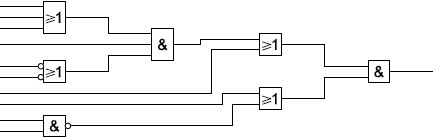
\includegraphics[width=0.3\textwidth]{pics/shanonursprung} & 
		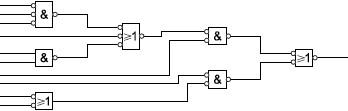
\includegraphics[width=0.3\textwidth]{pics/demorganende} &
		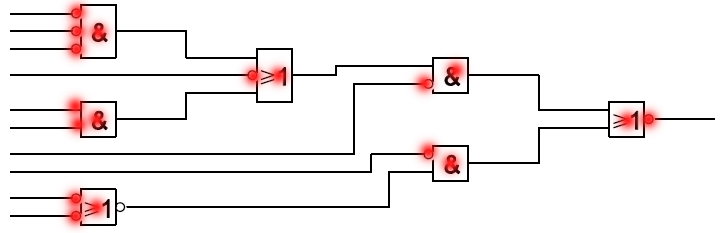
\includegraphics[width=0.3\textwidth]{pics/shanonende}\\
	 & DeMorgan	 &  Shannon \\
	 & $\neg(a \vee b) = \neg a \wedge \neg b$	&  $\neg f(a, b, c, ...z; \wedge, \vee) = f(\neg a, \neg v, \neg c, ... \neg z; \wedge, \vee)$ 
%		  $\neg(a \wedge b) = \neg a \vee \neg b $ \\ 
	\end{tabular}
% Die Negation einer beliebigen log. Funktion f erh"alt man, wenn man alle Variablen durch ihre Negation ersetzt und die Operatoren vertauscht. \\

\subsection{Normalformen: KDNF und KKNF}
	\begin{minipage}{10cm}
		Ausgangslage:\\
		\begin{tabular}{|l|l|l|l|l||l||l|}
			\hline	
				Dezimal & $x_2$ & $x_1$ & $x_0$ & y & DNF & KNF\\	
			\hline
			\hline
				0 & 0 & 0 & 0 & 0 & & $x_2 \vee x_1 \vee x_0$ \\
			\hline	
				1 & 0 & 0 & 1 & 1 &	$\overline{x_2} \wedge \overline{x_1} \wedge x_0$ & \\
			\hline
				2 & 0 & 1 & 0 & 0 & & $x_2 \vee \overline{x_1} \vee x_0$  \\
			\hline
				3 & 0 & 1 & 1 & 1 &	$\overline{x_2} \wedge x_1 \wedge x_0$ & \\
			\hline
				4 & 1 & 0 & 0 & 0 & & $\overline{x_2} \vee x_1 \vee x_0$ \\
			\hline
				5 & 1 & 0 & 1 & d & $[x_2 \wedge \overline{x_1} \wedge x_0]$ & $[\overline{x_2} \vee x_1 \vee \overline{x_0}]$  \\
			\hline
				6 & 1 & 1 & 0 & 1 & $x_2 \wedge x_1 \wedge \overline{x_0}$ &  \\
			\hline
				7 & 1 & 1 & 1 & 1 & $x_2 \wedge x_1 \wedge x_0$ &\\
			\hline
		\end{tabular}\\
	\newline
	
	\lbrack Don't care \rbrack = \lbrack d \rbrack
	
	\end{minipage}
\begin{minipage}{8cm}
\subsubsection{DNF} 
Kanonisch disjunktive Normalform (KDNF): Es werden nur diejenigen Zeilen der Wahrheitstabelle aufgef"uhrt, deren Funktionswert \textbf{1} oder \textbf{d} ist. \\
$y=(\overline{x_2} \wedge \overline{x_1} \wedge x_0) \vee (\overline{x_2} \wedge x_1 \wedge x_0) \vee [x_2 \wedge \overline{x_1} \wedge x_0] \vee (x_2 \wedge x_1 \wedge \overline{x_0}) \vee (x_2 \wedge x_1 \wedge x_0)$ \\

\subsubsection{KNF}
Kanonisch konjunktive Normalform (KKNF): 
Es werden nur diejenigen Zeilen der Wahrheitstabelle aufgef"uhrt, deren Funktionswert \textbf{0} oder \textbf{d} ist. \\
$y=(x_2 \vee x_1 \vee x_0) \wedge (x_2 \vee \overline{x_1} \vee x_0) \wedge (\overline{x_2} \vee x_1 \vee x_0) \wedge [\overline{x_2} \vee x_1 \vee \overline{x_0}]$ \\
\end{minipage}
\subsection{Karnaugh-Diagramm}
	\subsubsection{Arbeiten mit dem KV-Diagramm}
\begin{compactitem}
	\item 1) \ \ Aufstellen der Wahrheitstabelle.\\
	\item 2) \ \ "Ubertragen der Werte der Wahrheitstabelle ins KV Diagramm.\\
	\item 3) \ \ M"oglichst grosse Gruppen a $2^n$ Felder bilden (2, 4, 8 ...) (k"onnen auch "uber die Ecken gehen).\\
	\item 4)
	\begin{tabular}{ll}
		DNF: & KNF: \\
		Gruppen von Feldern mit Wert \textbf{1} oder \textbf{d} & Gruppen von Feldern mit Wert \textbf{0} oder \textbf{d}\\
		Primimplikanten: AND Verkn"upfung & Primimplikanten: OR Verkn"upfung\\
		OR Verkn"upfung aller Primimplikanten & AND Verkn"upfung aller Primimplikanten\\
	\end{tabular}
\end{compactitem}

\subsection{Karnaugh-Diagramm}
	\begin{multicols}{3}
		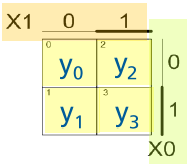
\includegraphics[width=0.3\textwidth]{pics/kv/2erKV} 
	\columnbreak
	
		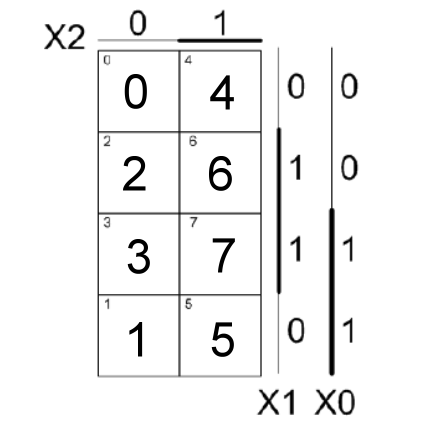
\includegraphics[width=0.3\textwidth]{pics/kv/3erKV}
	\columnbreak
	
		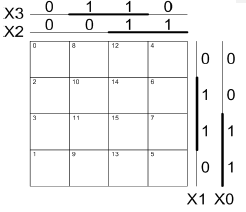
\includegraphics[width=0.3\textwidth]{pics/kv/4erKV}
	\end{multicols}
	
%	\subsubsection{Arbeiten mit dem KV-Diagramm}
%		\begin{compactitem}
%			\item 1) \ \ Aufstellen der Wahrheitstabelle.\\
%			\item 2) \ \ "Ubertragen der Werte der Wahrheitstabelle in KV Diagramm.\\
%			\item 3) \ \ M"oglichst grosse Gruppen a $2^n$ Felder bilden.\\
%			\item 4)
%				\begin{tabular}{ll}
%					Kanonisch disjunktive Normalform: & Kanonisch konjunktive Normalform: \\
%					Gruppen von Feldern mit Wert 1 oder d & Gruppen von Feldern mit Wert 0 oder d\\
%					Primimplikanten: AND Verkn"upfung & Primimplikanten: OR Verkn"upfung\\
%					OR Verkn"upfung aller Primimplikanten & AND Verkn"upfung aller Primimplikanten\\
%				\end{tabular}
%		\end{compactitem}